\section*{Приложение А\\(обязательное)\\Руководство пользователя}
\addcontentsline{toc}{section}{Приложение А (обязательное) Руководство пользователя}

Для начала работы с системой необходимо открыть веб-браузер, и подключиться по адресу http://<system\_ ip\_ addr>:9999.
После загрузки страницы, будет выведено окно входа (рисунок \ref{man_img:01}), с предложением ввести логин и пароль.\par

\begin{figure}[h!]
    \centering
    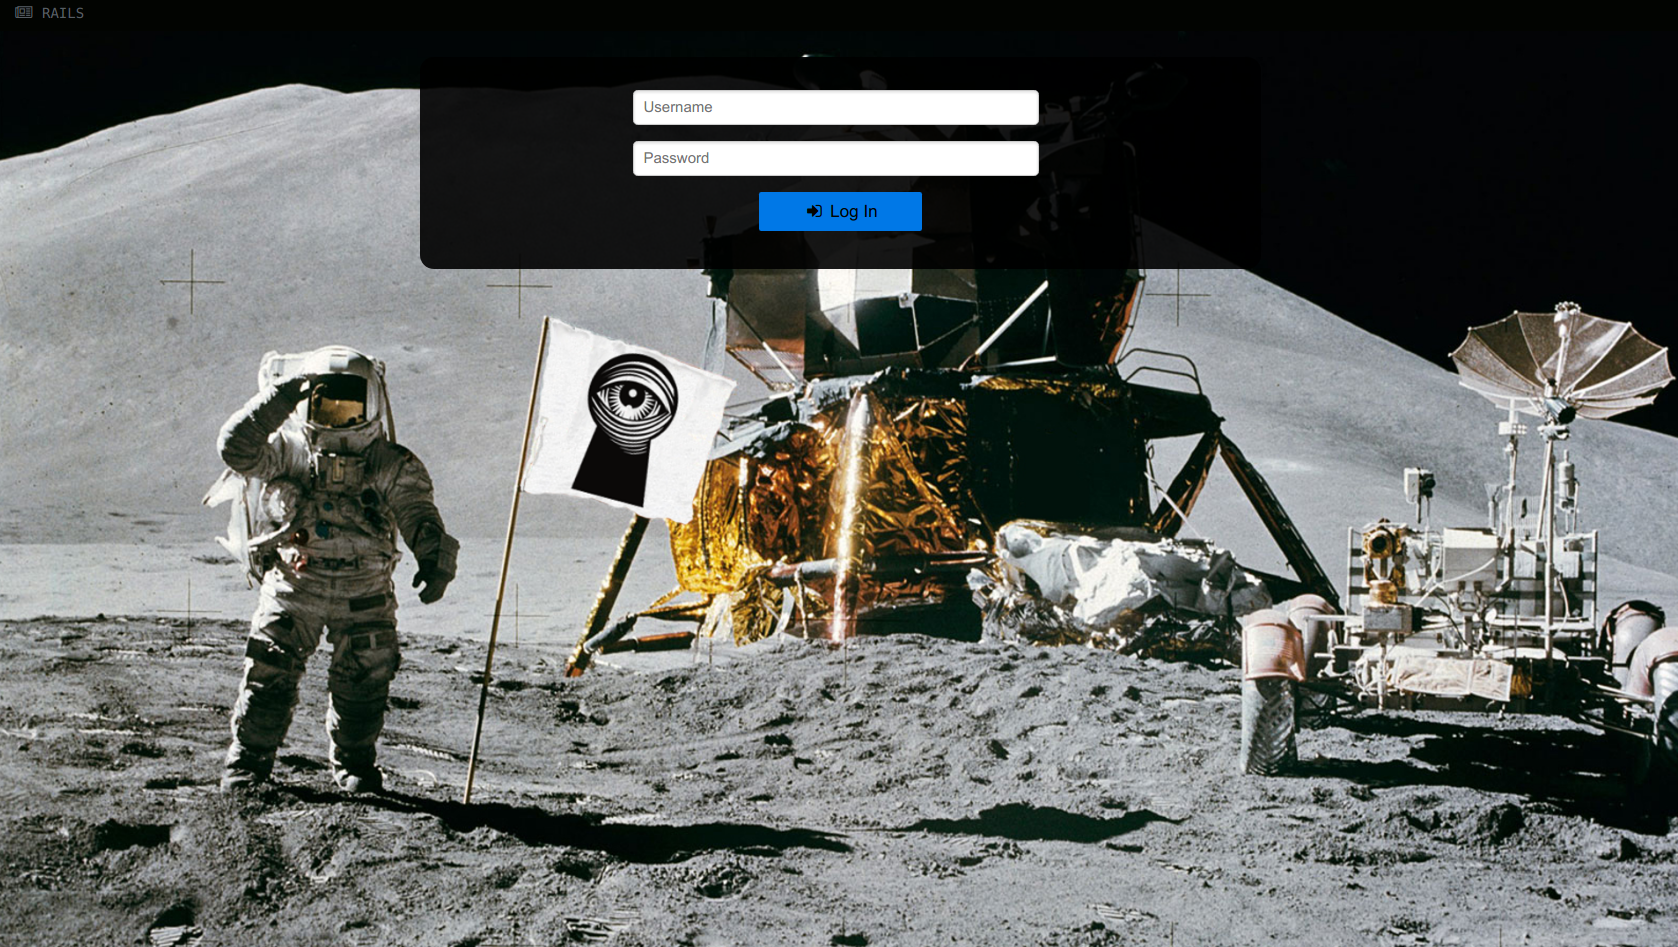
\includegraphics[width=0.7\textwidth]{man_01}
    \caption{Страница входа в систему}
    \label{man_img:01}
\end{figure}

Нажатие на кнопку <<Log In>> запускает процедуру входа в систему. При неправильно введённых логине/пароле пользователь будет перенаправлен на страницу с сообщением об ошибке (рисунок \ref{man_img:02}).\par

\begin{figure}[h!]
    \centering
    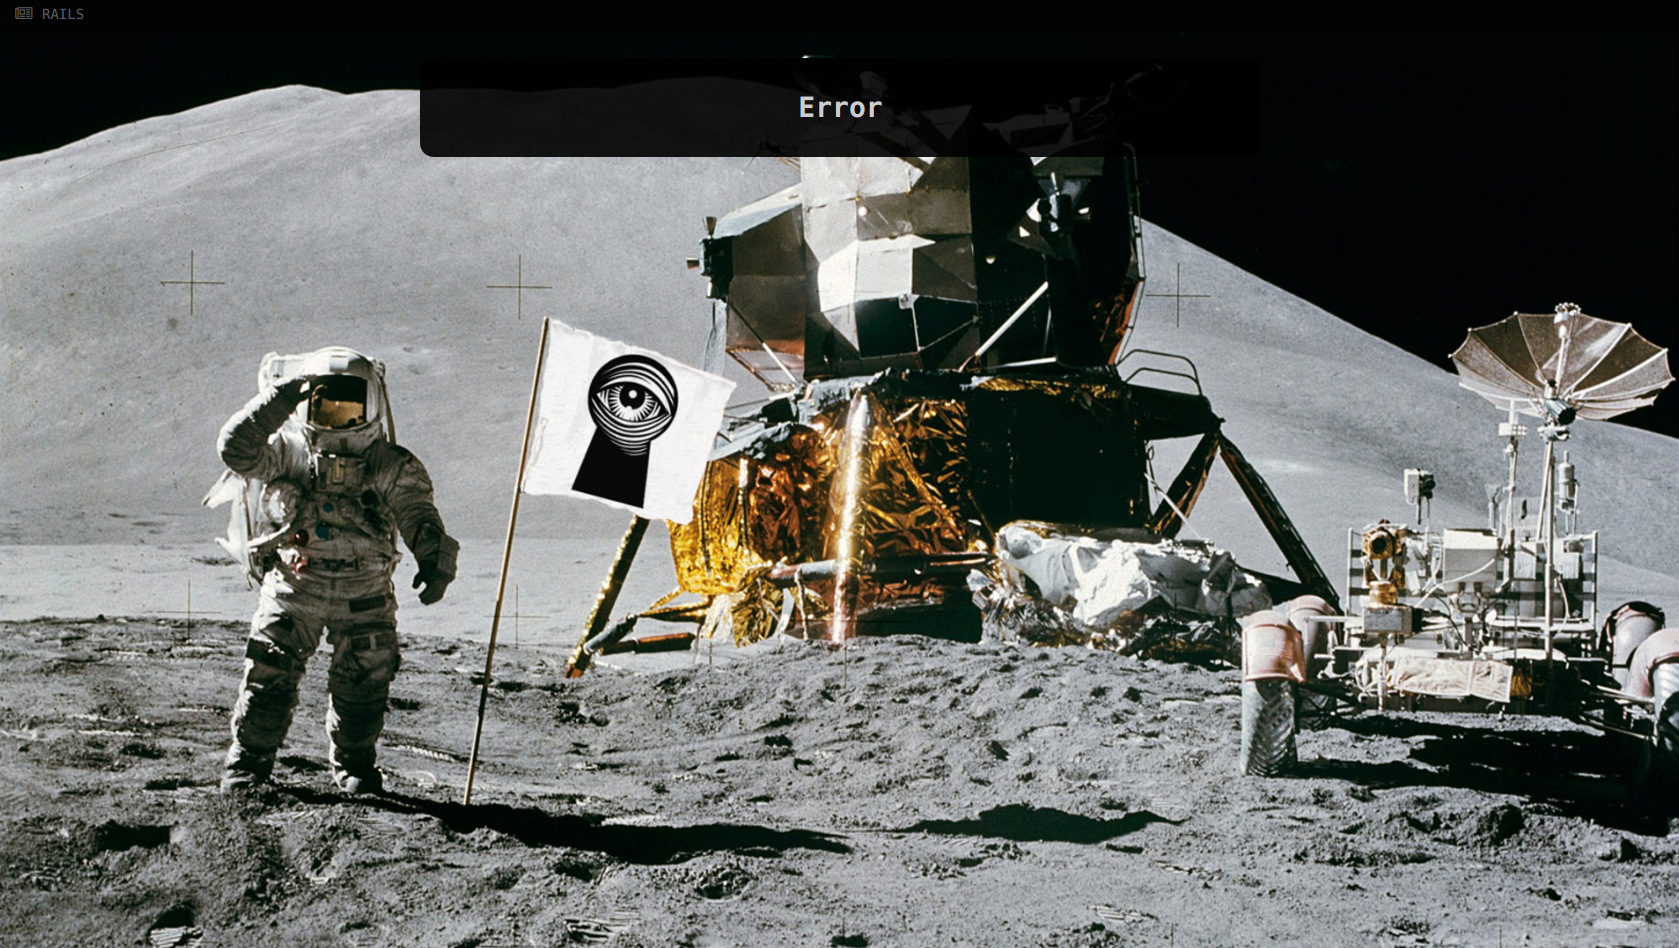
\includegraphics[width=0.7\textwidth]{man_02}
    \caption{Страница сообщения об ошибке}
    \label{man_img:02}
\end{figure}

Нажатие на кнопку <<Log In>> при корректно введённых логине и пароле приведёт к перенаправлению на основную страницу работы с системой (рисунок \ref{man_img:03}).\par

\begin{figure}[h!]
    \centering
    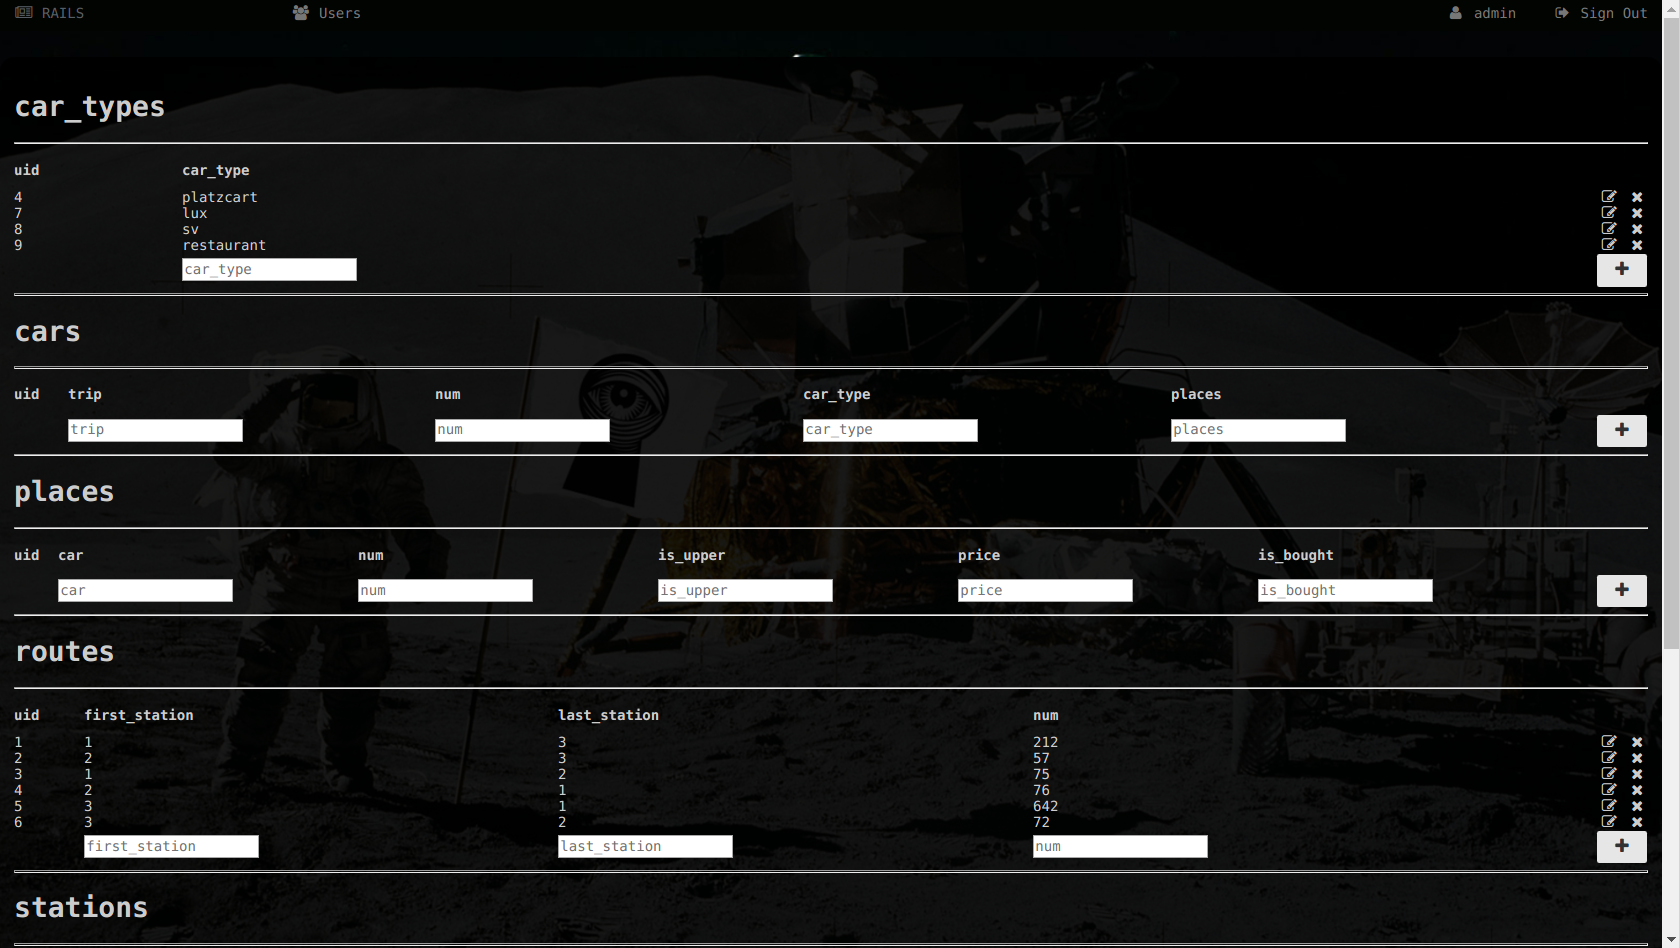
\includegraphics[width=0.7\textwidth]{man_03}
    \caption{Основная страница}
    \label{man_img:03}
\end{figure}

Вверху основной страницы (рисунок \ref{man_img:03}) расположена навигационная панель со следующими элементами (слева направо):
\begin{itemize}
    \item <<RAILS>> - ссылка на основную страницу;
    \item <<Users>> - ссылка на панель управления администратора (доступна только для пользователя admin);
    \item <<admin>> - имя пользователя, под которым осуществлён вход;
    \item <<Sign Out>> - кнопка для завершения сеанса текущего пользователя, и выхода из системы.
\end{itemize}

Центральное место на основной странице занимает интерфейс для работы с таблицами базы данных. Каждая пользовательская таблица базы данных представлена на странице следующими элементами управления (слева направо, сверху вниз):
\begin{itemize}
    \item название таблицы;
    \item строка с заголовками столбцов таблицы;
    \item содержимое таблицы, по строке на запись;
    \item форма создания новой записи таблицы.
\end{itemize}

Каждая запись таблицы представлена следующими элементами (слева направо):
\begin{itemize}
    \item значения полей записи;
    \item кнопка перехода на страницу редактирования записи;
    \item кнопка удаления записи.
\end{itemize}

Форма создания новой записи таблицы представлена следующими элементами:
\begin{itemize}
    \item поля для ввода текстовых данных, по полю на каждый столбец таблицы, за исключением столбца <<uid>>;
    \item кнопка добавления записи.
\end{itemize}

При нажатии на кнопку редактирования записи будет открыта страница редактирования данной записи (рисунок \ref{man_img:04}). При отсутствии соответствующих прав у текущего пользователя будет произведено перенаправление на страницу с сообщением об ошибке (рисунок \ref{man_img:02}.\par

При нажатии на кнопку удаления записи данная запись будет удалена. При отсутствии соответствующих прав у текущего пользователя будет произведено перенаправление на страницу с сообщением об ошибке (рисунок \ref{man_img:02}.\par

При нажатии на кнопку добавления записи будет создана запись таблицы с данными из полей ввода. При отсутствии соответствующих прав у текущего пользователя, или некорректно введённых данных будет произведено перенаправление на страницу с сообщением об ошибке (рисунок \ref{man_img:02}.\par

При нажатии на кнопку перехода к панели управления администратора будет осуществлён переход на страницу управления пользователями (рисунок \ref{man_img:05}). При отсутствии соответствующих прав у текущего пользователя будет произведено перенаправление на страницу с сообщением об ошибке (рисунок \ref{man_img:02}.\par

При нажатии на кнопку выхода из системы будет завершен сеанс текущего пользователя, и произведено перенаправление на страницу входа в систему (рисунок \ref{man_img:01}).\par

\begin{figure}[h!]
    \centering
    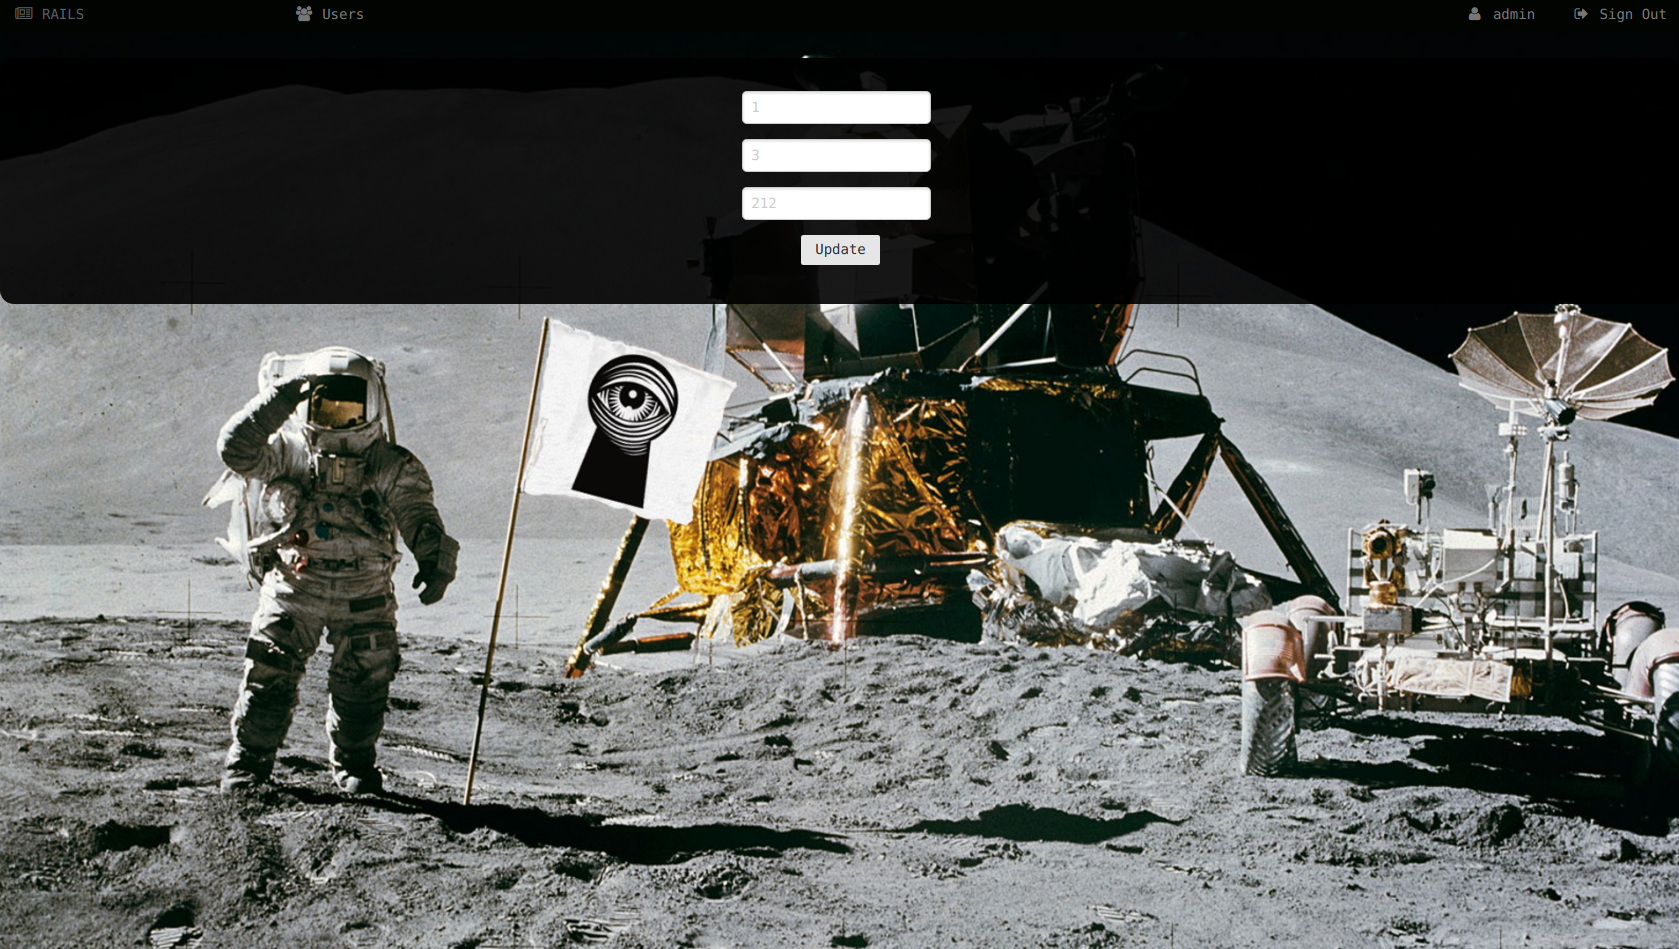
\includegraphics[width=0.7\textwidth]{man_04}
    \caption{Страница редактирования записи}
    \label{man_img:04}
\end{figure}

Страница редактирования записи (рисунок \ref{man_img:04}) представлена следующими элементами (сверху вниз):
\begin{itemize}
    \item навигационная панель, полностью аналогичная таковой на основной странице;
    \item поля редактирования записи, по полю на каждый столбец таблицы, за исключением столбца <<uid>>, заполненные соответствующими данными из таблицы;
    \item кнопка <<Update>>, вносящая изменения в базу данных.
\end{itemize}

При нажатии на кнопку внесения изменений изменённые данные записи будут внесены в таблицу, а пользователь будет перенаправлен на основную страницу (рисунок \ref{man_img:01}). При отсутствии соответствующих прав у текущего пользователя, или некорректно введённых данных будет произведено перенаправление на страницу с сообщением об ошибке (рисунок \ref{man_img:02}.\par

\begin{figure}[h!]
    \centering
    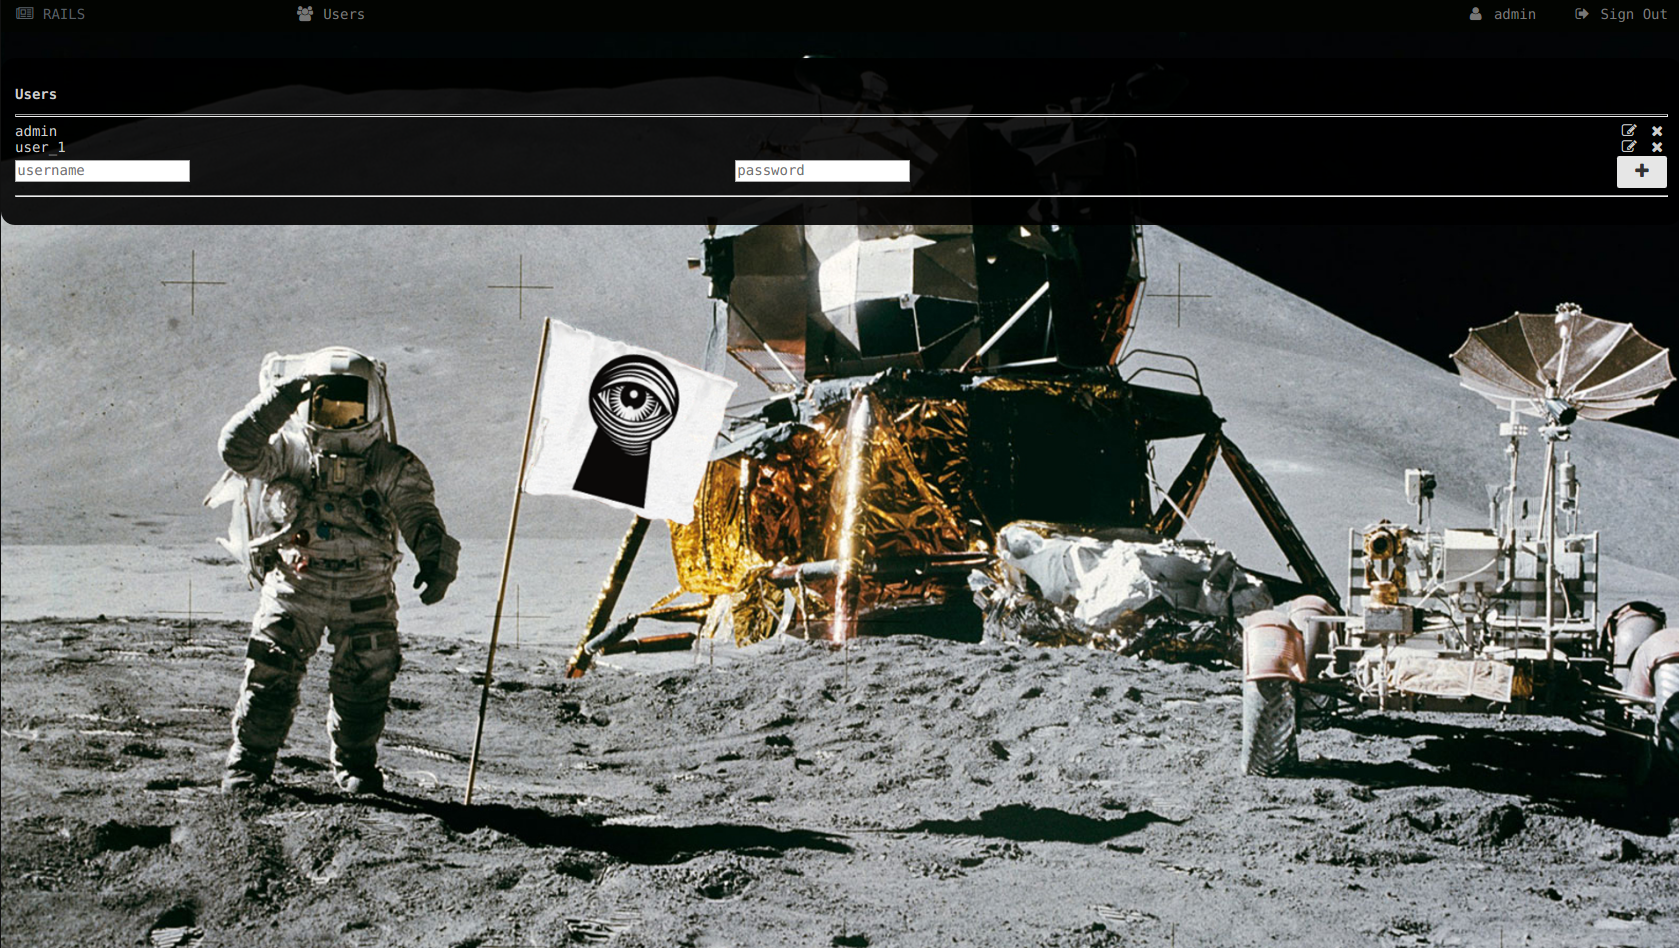
\includegraphics[width=0.7\textwidth]{man_05}
    \caption{Страница панели управления администратора}
    \label{man_img:05}
\end{figure}

Страница панели управления администратора (рисунок \ref{man_img:05}) представлена следующими элементами (сверху вниз):
\begin{itemize}
    \item навигационная панель, полностью аналогичная таковой на основной странице;
    \item список пользователей с кнопками для изменения и удаления каждого пользователя;
    \item форма создания нового пользователя.
\end{itemize}

При нажатии на кнопку редактирования пользователя будет открыта страница редактирования данного пользователя (рисунок \ref{man_img:06}). При отсутствии соответствующих прав у текущего пользователя будет произведено перенаправление на страницу с сообщением об ошибке (рисунок \ref{man_img:02}.\par

При нажатии на кнопку удаления пользователя данный пользователь будет удалён. При отсутствии соответствующих прав у текущего пользователя будет произведено перенаправление на страницу с сообщением об ошибке (рисунок \ref{man_img:02}.\par

При нажатии на кнопку добавления пользователя будет создан новый пользователь с логином и паролем из полей ввода. При отсутствии соответствующих прав у текущего пользователя, или некорректно введённых данных будет произведено перенаправление на страницу с сообщением об ошибке (рисунок \ref{man_img:02}.\par

\begin{figure}[h!]
    \centering
    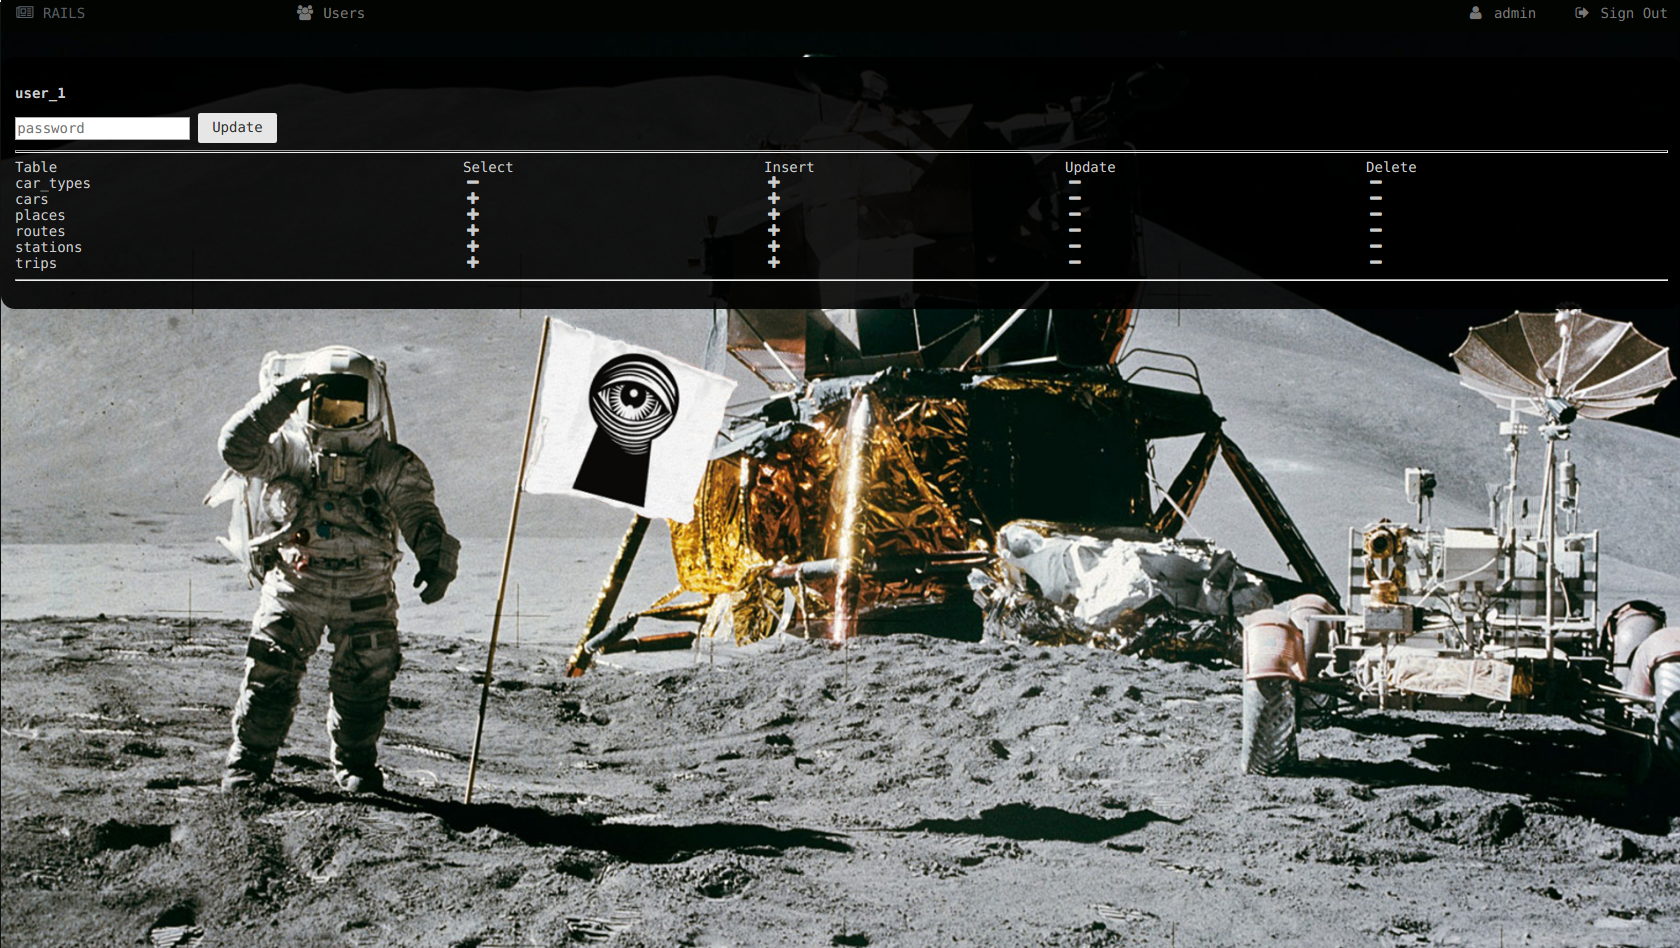
\includegraphics[width=0.7\textwidth]{man_06}
    \caption{Страница редактирования пользователя}
    \label{man_img:06}
\end{figure}

Страница редактирования пользователя (рисунок \ref{man_img:06}) представлена следующими элементами (сверху вниз, слева направо):
\begin{itemize}
    \item навигационная панель, полностью аналогичная таковой на основной странице;
    \item имя редактируемого пользователя;
    \item поле задания нового пароля пользователя;
    \item кнопка сохранения нового пароля;
    \item таблица разрешений пользователя.
\end{itemize}

При нажатии на кнопку <<Update>> данному пользователю будет установлен новый пароль из соответствующего поля ввода. При отсутствии соответствующих прав у текущего пользователя, или некорректно введённых данных будет произведено перенаправление на страницу с сообщением об ошибке (рисунок \ref{man_img:02}.\par

Таблица разрешений пользователя имеет следующую структуру:
\begin{itemize}
    \item в первом столбце содержатся имена пользовательских таблиц;
    \item во втором столбце содержатся маркеры наличия/отсутствия разрешения получения данных из соответствующих таблиц пользователем;
    \item в третьем столбце содержатся маркеры наличия/отсутствия разрешения добавления данных в соответствующие таблиц пользователем;
    \item в четвёртом столбце содержатся маркеры наличия/отсутствия разрешения изменения данных в соответствующих таблиц пользователем;
    \item в пятом столбце содержатся маркеры наличия/отсутствия разрешения удаления данных из соответствующих таблиц пользователем.
\end{itemize}

При нажатии на маркер наличия/отсутствия разрешения соответствующее разрешение у пользователя будет изменено на противоположное, а значение маркера будет обновлено. При отсутствии соответствующих прав у текущего пользователя будет произведено перенаправление на страницу с сообщением об ошибке (рисунок \ref{man_img:02}.\par
